
\documentclass[journal,11pt,onecolumn,draftclsnofoot]{ieeeconf}  % Comment this line out if you need a4paper

\usepackage{listings}
\usepackage{hyperref}
\usepackage{url}
\usepackage[pdftex]{graphicx}
\usepackage{amsfonts}
\usepackage{subfigure} 
\usepackage{algorithm}
%\usepackage{algorithmic}
\usepackage{amsmath}
\usepackage{bm}
\usepackage{algcompatible}
\usepackage{framed}
\usepackage{balance}

\usepackage{graphics} % for pdf, bitmapped graphics files
\usepackage{caption}
\usepackage{epsfig}
\usepackage{wrapfig}
\usepackage{breqn}
\newcommand{\myalpha}{\alpha_\rho}
\DeclareMathOperator*{\argmax}{arg\,max}

\pdfminorversion=4

\IEEEoverridecommandlockouts                              % This command is only needed if 
                                                          % you want to use the \thanks command
\overrideIEEEmargins                                      % Needed to meet printer requirements.

\author{Wenbo Xu, Wenwen Zhang, Yichi Zhang}

\title{
	EE 382C: Multicore Computing \protect\\
	\Large \bf Parallel GPU based Algorithms for Image Processing
}

\begin{document}
\maketitle
\thispagestyle{empty}
\pagestyle{empty}

\section{Introduction}
Recently, the requirement for GPU (graphics processing unit) performance as well as the computation speed are increasing rapidly. As comparison, GPU computation speed can be several times faster than traditional CPU. Moreover, as the programmability and parallel processing emerge\cite{1},  people began using GPU in some non-graphics applications, such as general-purpose computing on the GPU (GPGPU). To be more user-friendly, CUDA brings the C-like development environment and some CUDA extended libraries to programmers, which are based on industry-standard C/C++ and have straightforward APIs to manage devices, memory etc.

As a general use of GPU, image processing algorithms are always computationally expensive, however, parallel image processing algorithms can enhance the speed to a greater extent, especially for large-scale images.

In this paper, we realized Gaussian Filter in both CPU sequential logic and GPU parallel logic. Then, we implemented three improvements for GPU. By using cuda command line tool nvprof and the NVIDIA Visual Profiler, these optimizations have been proved to improve performance a lot.
\begin{figure}[h]

	\centering\includegraphics[width=85mm,height=70mm]{ImageProcessingCuda.png}
	\caption{Diagram for Parallel Image Processing}
	\label{parallel}
	\vspace*{-10mm}	
	
\end{figure}


\section{Gaussian blur}
\subsection{Definition and Usage}
In image processing, a Gaussian blur (also known as Gaussian smoothing) is the result of blurring an image by a Gaussian function. It is a widely used effect in graphics software, typically to reduce image noise and  detail. 

Mathematically, the Gaussian blur is a type of image-blurring filter that uses a Gaussian function for calculating the transformation to apply to each pixel in the image.  For our implementation, we use a two-dimension gaussian blur to filter each image pixel. The related two-dimension gaussian function is the product of two such one-dimension function above, on in each dimention. 
  \[G(x) = \frac{1}{ \sqrt{2 \pi   \sigma ^{2} } } e^{ -\frac{ x^{2} +  y^{2}}{2  \sigma ^{2} }}\]
 Variable $x$ is the distance from the origin in the horizontal axis, $y$ is the distance from the origin in the vertical axis, and $\sigma$ is the standard deviation of the Gaussian distribution. A convolution matrix is built with values generated by this distribution.  
 To have a better view of the powerfulness of parallel computing, we did a comparison experiment, which comprised of two implementations of Gaussian blur. One is sequential implementation and the other is parallel implementation. 

\subsection{Sequential  Implementation}\label{Sequential}
There are four steps of the sequential implementation. The first step is preprocess, which is responsible for reading image file and store it as Image class. The second step is to generate a gaussian filter, a matrix, based on parameters, like the standard deviation,  passed from users. The next step is to traverse each pixel in the image object and compute the values of a given pixel in the output image by multiplying each kernel value by the corresponding input image pixel values. The final step is to generate an image file from those new pixel values.

\subsection{Parallel  Implementation} \label{GPU}
In this section, we implemented a normal parallel version of gaussian blurring based on CUDA. In the following section, we optimized this implementation in several ways.  First, we read the image file and generate filter matrix. Then we copy the image into device memory. Each pixel is combined with three channels, $r$, $g$ and $b$.  They are separated and are gaussian blurred separately. Then we start the kernel three times and do gaussian blurring to each channel every time.  At last, we copy three blurred channels from device to host and save them into an image file. This process is described with the Fig.1.

\section{Optimization}

\subsection{Shared memory v.s. Global Memory} \label{shared}
In the previous version implementation of Gaussian blur, we store three channels in global memory, and access same global memory several times when we read neighbor channels. Since reading shared memory is much faster (shared memory $1.7TB/s$, while global memory $150GB/s$), instead of pulling from global memory every time, we put channel values in the shared memory for other threads within the same block to see and reuse. 

\begin{figure}[h]
	\centering\includegraphics[width=120mm,height=85mm]{SharedMemory.png}
	\caption{Loading neighbour channel values for shared variable}
	\label{parallel}
	\vspace*{-5mm}
\end{figure}
In order to compute blurred channel values at the boundary of one block, we need to load channel values from neighboring blocks, so shared memory size should be a little larger than a block size and threads at the boundary area are responsible for loading channel values from neighboring blocks. This is displayed in Fig.2. Threads in blue area of dotted rectangles are responsible for loading channel values from corresponding white area.

\subsection{Pageable v.s. Pinned Memory} \label{pinned}
Host data allocations are pageable by default, However, GPU cannot access data directly from pageable memory, but from pinned memory. As shown in Figure \cite{Mark}, whenever a data transfer is invoked on pageable memory, the CUDA driver has to allocate a temporary pinned memory array to copy host data and then transfer it to the device. \par
\begin{figure}[h]

	\centering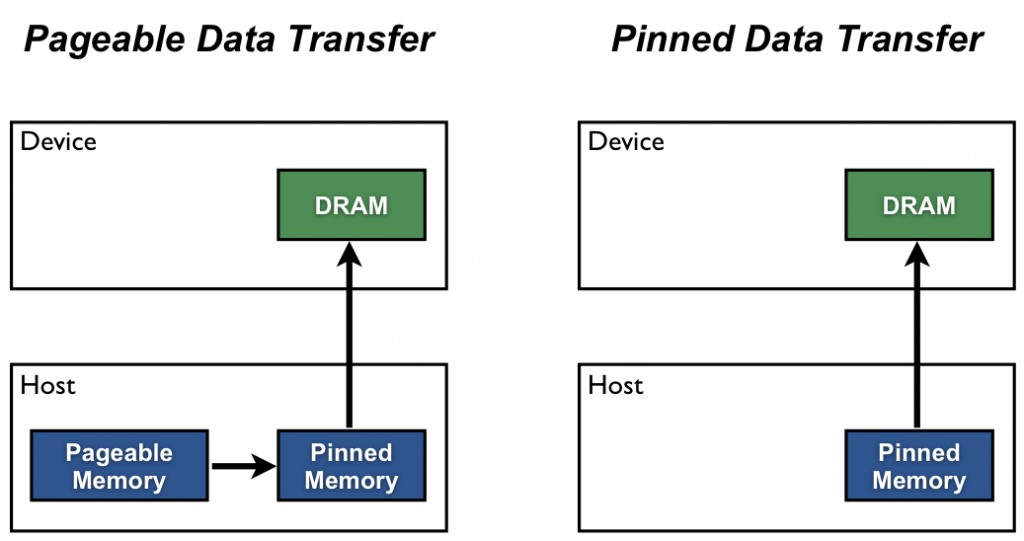
\includegraphics[width=120mm]{pinned.jpg}
	\caption{CUDA data transfer.\cite{Mark}}
	\label{CUDA data transfer.}
		\vspace*{-5mm}
\end{figure}
We can use \textit{cudaMallocHost()} and \textit{cudaFreeHost()} instead of \textit{malloc()} and \textit{free()}, to remove the overhead described above. However, \textit{cudaMallocHost()} and \textit{cudaFreeHost()} are more expensive with additional overheads. According to Boyer\cite{Trade_off}, pinned memory is faster when the size of data to be transfered is larger than 16MB. \par

\subsection{Streams} \label{stream}
A stream is defined as a sequence of operations in that execute in issue-order on the GPU. A typical CUDA task consists of three operations, memcpy HToD, kernel, and memcpyDToH. Kernel operations in different streams may run concurrently as long as the hardware resources were available. For memory copies, one transfer per direction is allowed at any time. And memory copies in different streams are in different direction may run concurrently when hardware supports two copy engine.   \par

Figure \ref{concurrent} illustrates the execution time line for three different scenarios. In this project, the pipelined fashion was implemented. In order to pipeline the memory copies, asynchronous memory copiy functions, \textit{cudaMemcpyAsync()}, are used instead of synchronous functions.\cite{Stream} \par

\section{Results}
Both CPU and GPU implementations was running on the TACC Stampede Supercomputer. The CPU is Intel® Xeon® E5-2680 2.7GHz Processors. And the GPU is NVIDIA K20 with 5120 MB GDDR5 memory and 2 copy engines. \par
The command line tool, nvprof, and the Nvidia Visual Profiler are used to profile the performance of our implementation. Profiling results are shown in Figure \ref{performances} and Figure \ref{table} in Appendix. In Figure \ref{performances} whith logarithmic scaled y axis,\\ 
1.�����	The CPU represents run time of a sequential CPU Gaussian filter as described in Section \ref{Sequential}.\\
2.�����	The stage1 represents the preliminary GPU parallel Gaussian filter as described in Section \ref{GPU}.\\
3.�����	The stage2 represents the GPU parallel Gassian filter with pipelined optimization as described in Section \ref{pinned} and \ref{stream}.\\
4.�����	The stage3 represents the GPU with shared memory as described in Section \ref{shared} additional to the optimization of stage2.\\

\begin{figure}[h]
		\vspace*{-5mm}
	\fbox{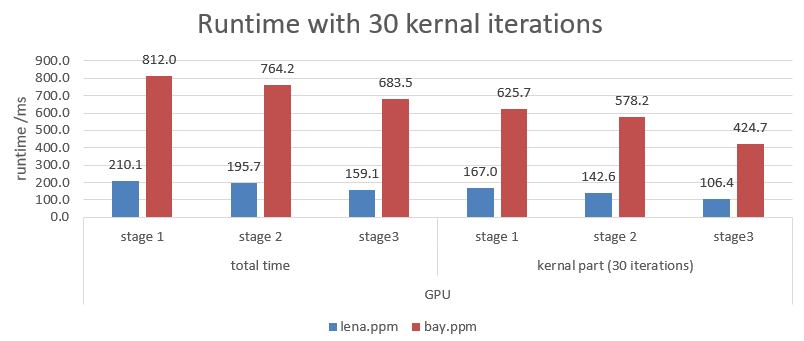
\includegraphics[width=160mm, height=60mm]{chart.PNG}}
	\caption{Performance Improvement in GPU.}
	\label{performances}
	\vspace*{-5mm}
\end{figure}
Each of the algorithm listed above will be running with two images: lena.ppm with $(512*512)$ pixels, and bay.ppm with $(1024*1024)$ pixels. For each algorithm, the kernel section, which contains memcpy HToD, actual Gaussian kernel, and memcpy DToH for GPU based algorithms, will be executed 30 consecutive times for better comparison between different stages. The duration of overall execution and Gaussian blur are both profiled. \par

The visual profiler timeline of the stage1 and stage3 are shown in Figure \ref{viewer}. The timescale of the two timelines are the same. The length difference of the green bars demonstrates the improvement for the kernel executions. There is approximated of 40\% improvement when the shared memory for GPU is implemented. And the stage3 with three streams, which are run in a pipelined fashion, and overlapping of kernel operations can be observed. However, the overlapping of kernels doesn't indicate of ture concurrency as described in Figure \ref{concurrent}. This is due to the limitation of the hardware resource. The number of blocks can be schedule on GPU is limited. For NVIDIA K20, this limitation is 180 blocks. Whenever this limit is reached, kernels has to wait for next free block.

\begin{figure}[!tbp]
	\centering
	\vspace*{-5mm}
	\begin{minipage}[b]{1\textwidth}
		\fbox{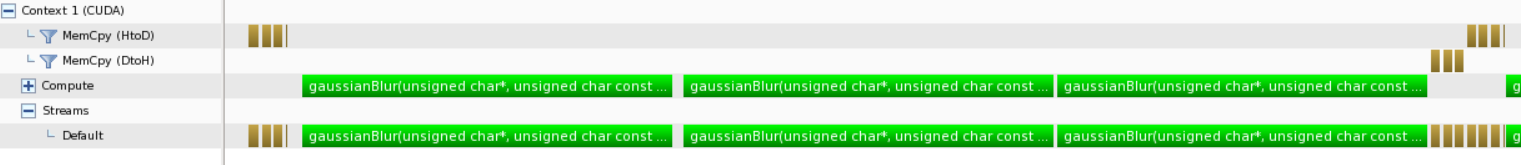
\includegraphics[width=160mm, height=40mm]{stage1.PNG}}
	\end{minipage}
	\begin{minipage}[b]{1\textwidth}
		\boxed{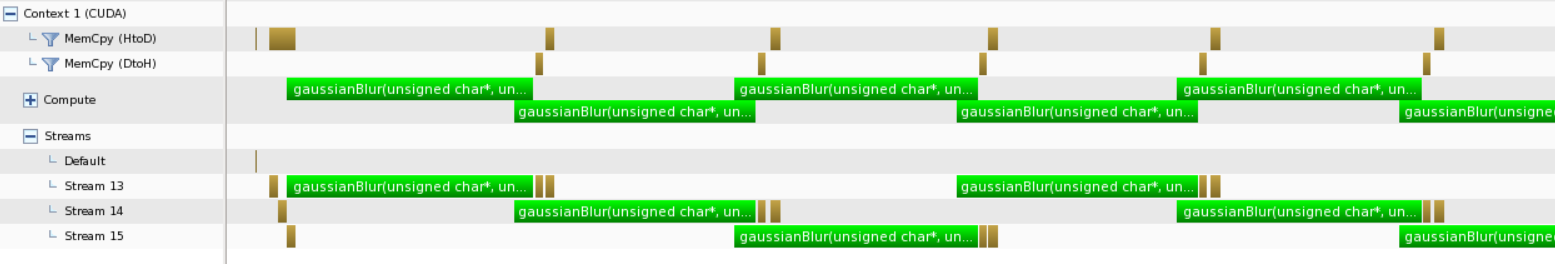
\includegraphics[width=160mm, height=60mm]{stage3.PNG}}
	\end{minipage}
	
	\caption{Time profiler viewer without using streams(top) verses using streams(bottom)}
	\label{viewer}
	\vspace*{-5mm}
\end{figure}

\section{Conclusion} 
In this project, we implemented a parallel GPU based Gaussian filter. The GPU based algorithm is benchmarked with two images, $(512*512)$ and $(1024*1024)$ pixels, and compared with performance of a sequential CPU based algorithm. The GPU based algorithm is optimized with three methods: \\
1.����� Memory allocation changed from pageable memory to pinned memory to reduce overhead\\
2.����� Stream sequences to allow operations run in pipelined fashion \\
3.����� Shared memory inside kernels to improve kernel memory access bandwidth\par

As shown above, the kernel part time with image lena.ppm for CPU sequential algorithm is 16.4s. This time is improved to 167.0ms with the preliminarily GPU based algorithm, which yields to a speed up of 98.2x. Ultimately, the stage3 achieved a speed up of 156.0x.

\clearpage
\appendix
\section{Appendix}
\begin{figure}[h]
	\centering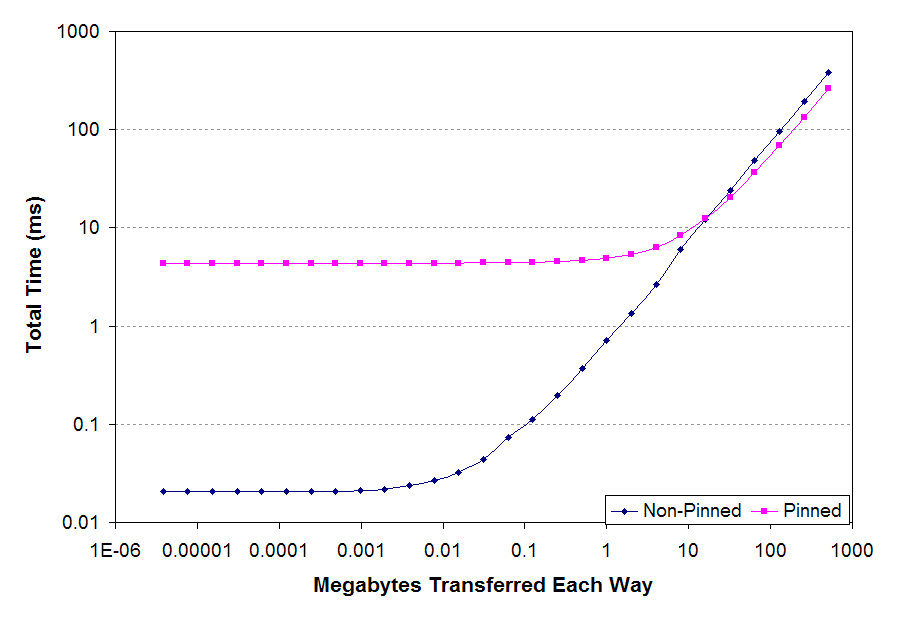
\includegraphics[width=120mm]{pinned_trade_off.png}
	\caption{Time required to allocate, transfer to the GPU, transfer back to the CPU, and deallocate pinned and non-pinned memory.\cite{Trade_off}}
	\label{Time required to allocate, transfer to the GPU, transfer back to the CPU, and deallocate pinned and non-pinned memory.}
\end{figure}
\begin{figure}[h]
	\centering
	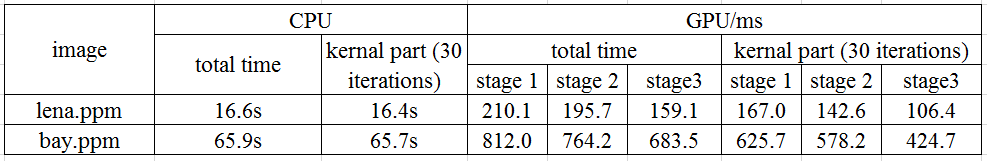
\includegraphics[width=170mm]{table.png}
	\caption{Performance Profiling Chart}
	\label{table}
\end{figure}
\begin{figure}[h]
	\centering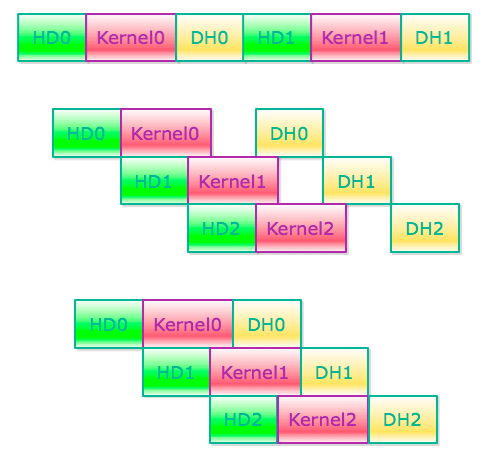
\includegraphics[width=120mm]{concurrent.png}
	\caption{Top: all operation in default stream. Mid: concurrent streams with one copy engine. Bottom: concurrent streams with two copy engine.}
	\label{concurrent}
\end{figure}

\clearpage
\bibliographystyle{abbrv}
\begin{thebibliography}{9}
\bibitem{1}
WU En Hua , ?State of the Art and Future Challenge on General 
Purpose Computation by Graphics Processing Unit?, Journal of 
Software, vol. 15, no. 10, 2004,pp.1493~1504.

\bibitem{Mark} 
Harries, M. (2012, December). How to Optimize Data Transfers in CUDA C/C++. Retrieved from https://devblogs.nvidia.com/parallelforall/how-optimize-data-transfers-cuda-cc/
	
\bibitem{Trade_off} 
Boyer, M. Choosing Between Pinned and Non-Pinned Memory. Retrieved from https://www.cs.virginia.edu/~mwb7w/cuda_support/pinned_tradeoff.html
	
\bibitem{Stream} 
Harries, M. (2012, December). How to Overlap Data Transfers in CUDA C/C++. Retrieved from https://devblogs.nvidia.com/parallelforall/how-overlap-data-transfers-cuda-cc/
	

\end{thebibliography}

\end{document}